\graphicspath{{./figures}}

\section{RF Module}

\subsection{Setup}
The radio module and communication link were initially tested/characterised using two small, off-the-shelf helical antennas, before integrating the custom-built antennas. The helical antennas managed an initial range of around 50 m in an urban area with a LoRa spreading factor of 8. This was tested with the one antenna near a window indoors, and the second antenna inside a car. This test served merely as a "proof-of-concept", and was not intended as an indication of system performance.

\subsection{Transmit Power Consumption}
The custom-built antennas were then connected to both the PQ and the GS and more detailed tests were conducted. The first test measured the power consumption for the PQ unit as a function of transmit power. This is displayed in Figure \ref{fig:txPower}, after subtracting a 31 mA "no-transmit" current. The maximum current is around 96 mA for the maxium output power (quoted by the RA-02 as 18 dBm +- 1 dBm).

\begin{figure}[!htb]
  \centering
  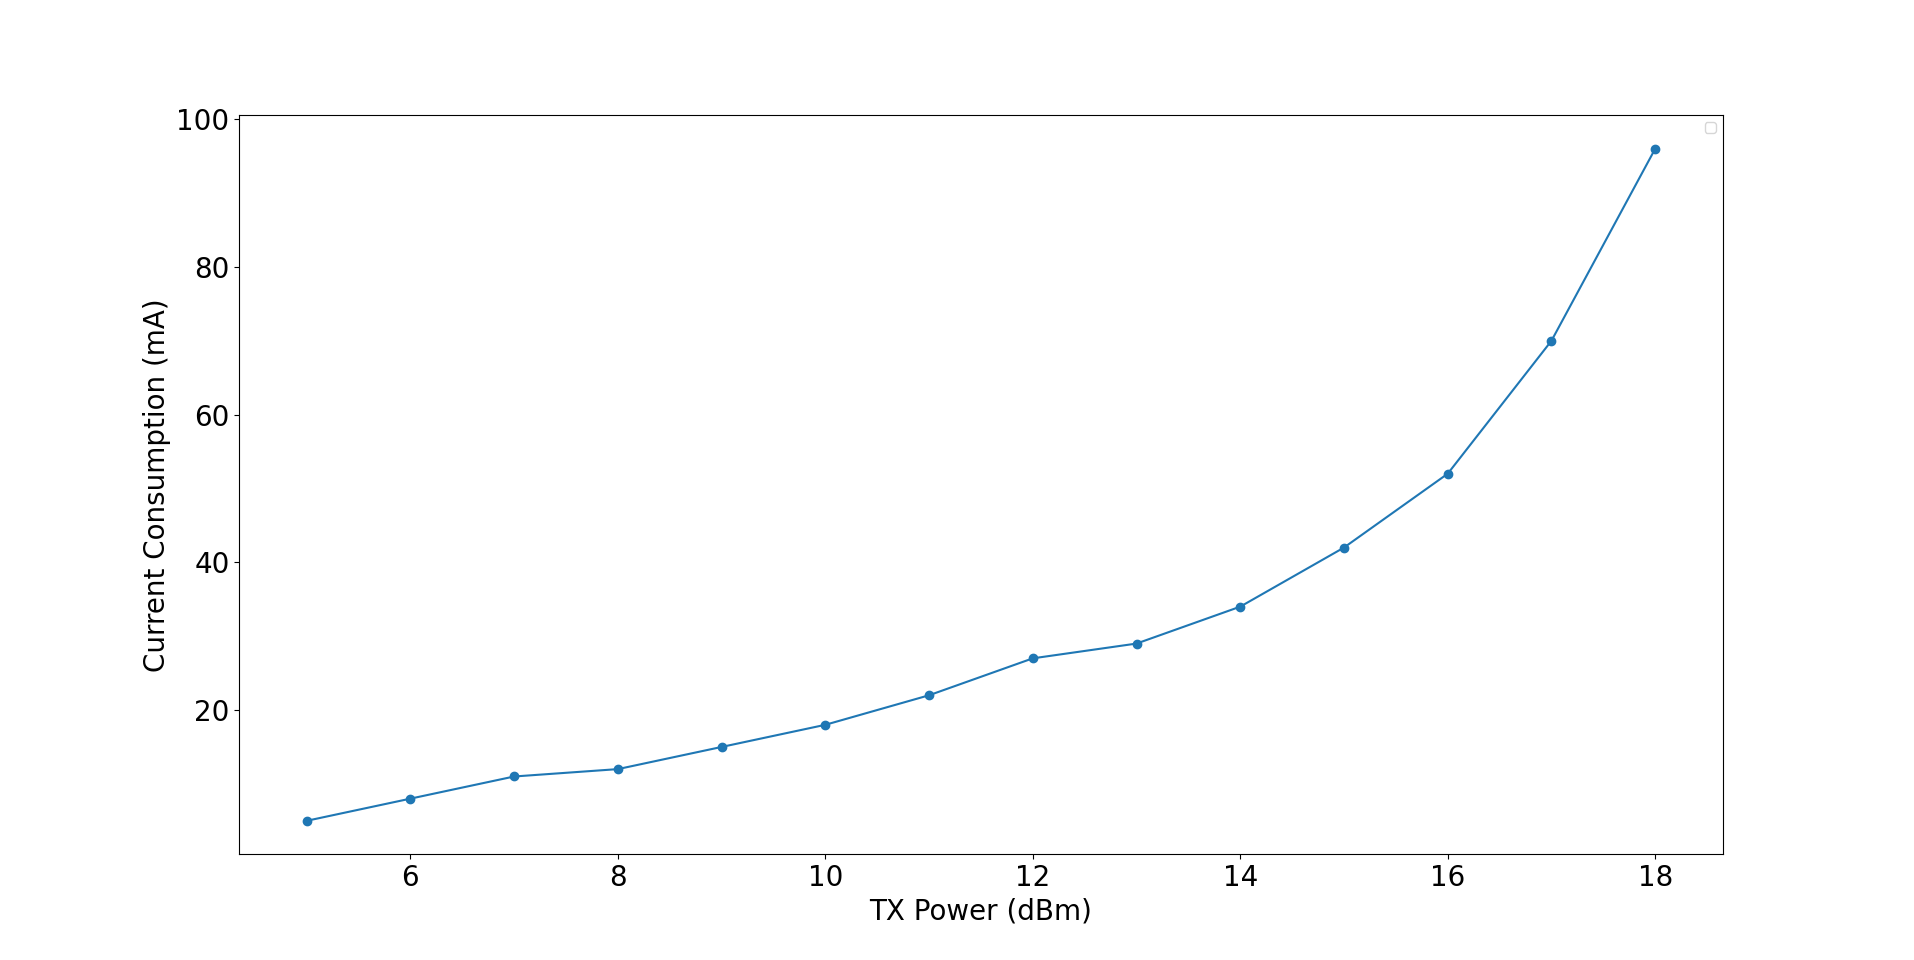
\includegraphics[width=0.85\textwidth]{txPower}
  \caption{TX Output Power vs Current Consumption}
  \label{fig:txPower}
\end{figure}

\subsection{Data Rate}
To test the possible bit rates as a function of LoRa spreading factor (SF), two RA-02 modules were setup with the same parameters and the bit rate was measured as the SF value was varied. A payload length of 255 was used, with 4/6 CRC, an 8 bit preamble, 500 kHz bandwidth, and a 10 ms delay between packets. The bit rate was then measured on the receiving side and is shown in Table \ref{tab:loraBitRate}.

\begin{table}[!htb]
  \centering
  \renewcommand{\arraystretch}{1.2}
  \begin{tabular}{ |c|c|c| }
  \hline
  \textbf{Spreading Factor}        & \textbf{Theoretical Bit Rate (bps)}      & \textbf{Measured Bit Rate (bps)}    \\
  \hline
  7         & 18229         & 17200       \\  \hline
  8         & 10417         & 10240       \\  \hline
  9         & 5859          & 5800        \\  \hline
  10        & 3255          & 3320        \\  \hline
  11        & 1790          & 1846        \\  \hline
  \end{tabular}
  \caption{LoRa Bit Rate vs Spreading Factor}
  \label{tab:loraBitRate}
\end{table}

The results show that the system is set up correctly, and that a spreading factor of 8 is the correct choice to achieve the 9600 baud rate requirement.